\documentclass[compress]{beamer}
\usepackage{ifthen,verbatim}

\newcommand{\isnote}{}
\xdefinecolor{lightyellow}{rgb}{1.,1.,0.25}
\xdefinecolor{darkblue}{rgb}{0.1,0.1,0.7}

%% Uncomment this to get annotations
%% \def\notes{\addtocounter{page}{-1}
%%            \renewcommand{\isnote}{*}
%% 	   \beamertemplateshadingbackground{lightyellow}{white}
%%            \begin{frame}
%%            \frametitle{Notes for the previous page (page \insertpagenumber)}
%%            \itemize}
%% \def\endnotes{\enditemize
%% 	      \end{frame}
%%               \beamertemplateshadingbackground{white}{white}
%%               \renewcommand{\isnote}{}}

%% Uncomment this to not get annotations
\def\notes{\comment}
\def\endnotes{\endcomment}

\setbeamertemplate{navigation symbols}{}
\setbeamertemplate{headline}{\mbox{ } \hfill
\begin{minipage}{5.5 cm}
\vspace{-0.75 cm} \small
\end{minipage} \hfill
\begin{minipage}{4.5 cm}
\vspace{-0.75 cm} \small
\begin{flushright}
\ifthenelse{\equal{\insertpagenumber}{1}}{}{Jim Pivarski \hspace{0.2 cm} \insertpagenumber\isnote/\pageref{numpages}}
\end{flushright}
\end{minipage}\mbox{\hspace{0.2 cm}}\includegraphics[height=1 cm]{../cmslogo} \hspace{0.1 cm} \includegraphics[height=1 cm]{../tamulogo} \hspace{0.01 cm} \vspace{-1.05 cm}}

\begin{document}
\begin{frame}
\vfill
\begin{center}
\textcolor{darkblue}{\Large Measuring {\it Differences} in Momentum Scale \\ \vspace{0.2 cm} as a Function of Track Parameters}

\vfill
\begin{columns}
\column{0.3\linewidth}
\begin{center}
\large
\textcolor{darkblue}{Jim Pivarski}
\end{center}
\end{columns}

\begin{columns}
\column{0.3\linewidth}
\begin{center}
\scriptsize
{\it Texas A\&M University}
\end{center}
\end{columns}

\vfill
 ? March, 2010

\end{center}
\end{frame}

%% \begin{notes}
%% \item This is the annotated version of my talk.
%% \item If you want the version that I am presenting, download the one
%% labeled ``slides'' on Indico (or just ignore these yellow pages).
%% \item The annotated version is provided for extra detail and a written
%% record of comments that I intend to make orally.
%% \item Yellow notes refer to the content on the {\it previous} page.
%% \item All other slides are identical for the two versions.
%% \end{notes}

\small

\begin{frame}
\frametitle{Motivation}
\begin{itemize}
\item Alignment optimizes tracks very well locally, but less so globally
\begin{itemize}
\item any two regions that are rarely crossed by the same track can
  develop different momentum scales through weak modes
\end{itemize}
\item Masses of $J/\psi$, $\Upsilon$, and $Z$ set the momentum scale,
  but with some complications
\begin{itemize}
\item each daughter samples a different region of the tracker: needs to be untangled
\item shape is not symmetric due to final state radiation
\item backgrounds must be part of the fit
\end{itemize}
\item In this talk, I'll present a procedure that can equalize
  momentum scales in all regions of the tracker, but not set the absolute scale
\item How it fits into a complete track-correction program:
\begin{center}
alignment $\to$ this correction $\to$ absolute scale correction
\end{center}
\item Also provides uncertainties and correlations in the remaining bias,
  which are important for setting systematic errors on physics quantities
\end{itemize}
%% \hspace{-0.83 cm} \textcolor{darkblue}{\Large Outline2}
\end{frame}

\begin{frame}
\frametitle{The idea}

\begin{itemize}
\item Alignment makes module positions and track parameters mutually
  consistent (optimizes track shapes)
\item Overall momentum scale correction adjusts observed resonance
  peaks to externally known values
\item Another physics constraint: momentum direction of daughters of a
  decay-in-flight must be consistent with the flight direction

\begin{center}
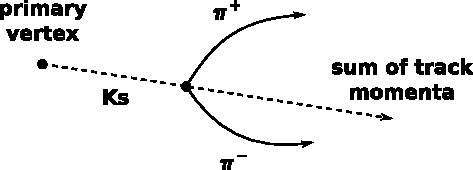
\includegraphics[width=0.5\linewidth]{diagram.pdf}
\end{center}

\vspace{-0.5 cm}
\begin{itemize}
\item sensitive to different momentum scales in different regions of the detector, but not absolute scale
\item symmetric in the case of no misalignment (unlike mass peak)
\end{itemize}

\item $K_S \to \pi^+\pi^-$ for low momenta, perhaps $B \to$ ``all charged'' for \mbox{higher?\hspace{-1 cm}}
\begin{itemize}
\item boosted $K_S$ are not sufficient because we need the daughters to sample different parts of the detector: need high mass
\end{itemize}
\end{itemize}
\end{frame}

\begin{frame}
\frametitle{Untangling daughters (1/2)}

\begin{itemize}
\item Same formalism as alignment (HIP for a single alignable):
\begin{center}
$\mbox{($N$ track residuals)} = \mbox{(6$\times N$ matrix)} \cdot \mbox{(6-DOF parameters)}$
\end{center}

\item $N$ decays with angle difference $\Delta \vec{\phi}$, track-parameter
  corrections described by $M$ parameters $\vec{p}$ ($N \gg M$):
\begin{center}
$\left(\begin{array}{c}\Delta \phi_1 \\ \vdots \\ \Delta \phi_N \end{array}\right) = A \cdot \left(\begin{array}{c}p_1 \\ \vdots \\ p_M \end{array}\right)$
\end{center}

\item $A$ is the transformation from parameters $\vec{p}$ to
  observables $\Delta \vec{\phi}$ and is therefore the derivative
  $\frac{\partial \left(\Delta \phi_i \right)}{\partial p_j}$, which can be computed \mbox{numerically:\hspace{-1 cm}}
\begin{enumerate}\setlength{\itemsep}{0.2 cm}
\item for each decay $i$, compute nominal $\Delta \phi_i$
\item for each parameter $j$, apply $\epsilon p_j$ to all tracks for $\Delta \phi_i(\epsilon p_j)$
\item $\displaystyle A_{ij} = \frac{\Delta \phi_i - \Delta \phi_i(\epsilon p_j)}{\epsilon}$
\end{enumerate}
\end{itemize}
\end{frame}

\begin{frame}
\frametitle{Untangling daughters (2/2)}
\begin{itemize}\setlength{\itemsep}{0.25 cm}
\item The values of $\vec{p}$ which minimize quadratic $\chi^2$ \mbox{(assumes Gaussian $\Delta \vec{\phi}$)\hspace{-1 cm}}
\begin{center}
$\chi^2 = \left( \Delta \vec{\phi} - A \cdot \vec{p} \right)^T \left( {\sigma_{\Delta \phi}}^2 \right)^{-1} \left( \Delta \vec{\phi} - A \cdot \vec{p} \right)$
\end{center}
are $\vec{p} = \left( A^T \left( {\sigma_{\Delta \phi}}^2 \right)^{-1} A \right)^{-1} \left( A^T \left( {\sigma_{\Delta \phi}}^2 \right)^{-1} \Delta \vec{\phi} \right)$ \hfill $\sim \frac{\sum w_i x_i}{\sum w_i}$

\vspace{0.25 cm}
with uncertainty/covariance $\left( A^T \left( {\sigma_{\Delta \phi}}^2 \right)^{-1} A \right)^{-1}$ \hfill $\sim \frac{1}{\sum w_i}$

\begin{itemize}\setlength{\itemsep}{0.1 cm}
\item ``convert $\Delta \vec{\phi}$ into $\vec{p}$ space and compute weighted mean''

\item the ${\sigma_{\Delta \phi}}^2$ weights are propagated uncertainties in $\Delta \vec{\phi}$
\end{itemize}

\item The final $\vec{p}$ correct biases in tracking, but perhaps more
  importantly, the covariance provides a rigorous systematic error in tracking

\item Potential early application: $\Xi^\pm$ mass measurement; tracking bias is the only systematic error
\end{itemize}
\end{frame}

\begin{frame}
\frametitle{Parameterization of $\vec{p}$}
\begin{itemize}
\item Biases are small and slowly varying (largest alignment weak modes are global distortions)

\item Expand general $\vec{p}(\phi, \kappa, \cot\theta, d_{xy}, d_z)$ function and keep low-order
\begin{itemize}
\item Fourier-expand in $\phi$: $\sin\phi$, $\cos\phi$, $\sin 2\phi$, $\cos 2\phi$
\item Taylor-expand in other parameters: $\kappa$, $\kappa\cot\theta$, $(\cot\theta)^2$
\item $\kappa$ and $d_{xy}$ are not sampled near zero due to physics
  signature: exclude $\kappa^2$ and ${d_{xy}}^2$ terms
\end{itemize}

\item 33 terms for $\delta \kappa$

\vspace{-0.5 cm}
{\scriptsize \begin{multline*}
\delta \kappa = 
p_{1} +
p_{2} \sin(\phi) +
p_{3} \cos(\phi) +
p_{4} \sin(2 \phi) +
p_{5} \cos(2 \phi) + \\
p_{6} \kappa +
p_{7} \cot\theta +
p_{8} d_{xy} +
p_{9} d_z +
p_{10} \sin(\phi) \kappa + \\
p_{11} \sin(\phi) \cot\theta +
p_{12} \sin(\phi) d_{xy} +
p_{13} \sin(\phi) d_z +
p_{14} \cos(\phi) \kappa +
p_{15} \cos(\phi) \cot\theta + \\
p_{16} \cos(\phi) d_{xy} +
p_{17} \cos(\phi) d_z +
p_{18} \sin(2 \phi) \kappa +
p_{19} \sin(2 \phi) \cot\theta +
p_{20} \sin(2 \phi) d_{xy} + \\
p_{21} \sin(2 \phi) d_z +
p_{22} \cos(2 \phi) \kappa +
p_{23} \cos(2 \phi) \cot\theta +
p_{24} \cos(2 \phi) d_{xy} +
p_{25} \cos(2 \phi) d_z + \\
p_{26} \kappa \cot\theta +
p_{27} \kappa d_{xy} +
p_{28} \kappa d_z +
p_{29} \cot\theta \cot\theta + \\
p_{30} \cot\theta d_{xy} +
p_{31} \cot\theta d_z +
p_{32} d_{xy} d_z +
p_{33} d_z d_z
\end{multline*}}

\vspace{-0.5 cm}
\item Same for $\delta \phi$ and $\delta d_{xy}$: 99 parameters, $99\times 99$ matrix inversion

\item $\delta \cot\theta$ and $\delta d_z$ cannot be optimized; used to select primary vertex
\end{itemize}
\end{frame}

\begin{frame}
\frametitle{$K_S \to \pi^+\pi^-$ selection}
\begin{itemize}\setlength{\itemsep}{0.25 cm}
\item Identify $K_S \to \pi^+\pi^-$ by $\pi^+\pi^-$ invariant mass \\ (it therefore cannot be used in the optimization)

\item Use sideband for a background control sample; sideband events
  enter the minimization with negative weight, cancelling the effect
  of backgrounds under mass peak

\item Identify the correct primary vertex by propagating $K_S$ to beamline in $r-z$ plane ($\delta \cot\theta$ and $\delta d_z$ cannot be optimized)

\begin{center}
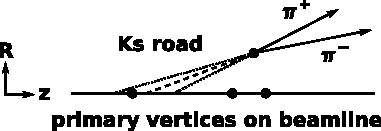
\includegraphics[width=0.4\linewidth]{diagram2.pdf}
\end{center}

\item Require exactly one primary vertex in the road from $K_S$

\item Require $K_S$ vertex to be within $1.5 < |v_{xy}| < 3$~cm; away
  from beamspot and within first pixel layer

\item From $K_S \to \pi^+\pi^-$, typical curvatures are $0.5 \lesssim |\kappa| \lesssim 5$~GeV$^{-1}$
\end{itemize}
\end{frame}

%% \section*{First section}
%% \begin{frame}
%% \begin{center}
%% \Huge \textcolor{blue}{First section}
%% \end{center}
%% \end{frame}

\begin{frame}
\frametitle{Feasibility study (1/6)}
\begin{itemize}
\item Quick check to make sure that there aren't any show-stoppers
\item MC and 1$^{\mbox{st}}$ RECO data (non-optimal tracking: large APEs)
\end{itemize}

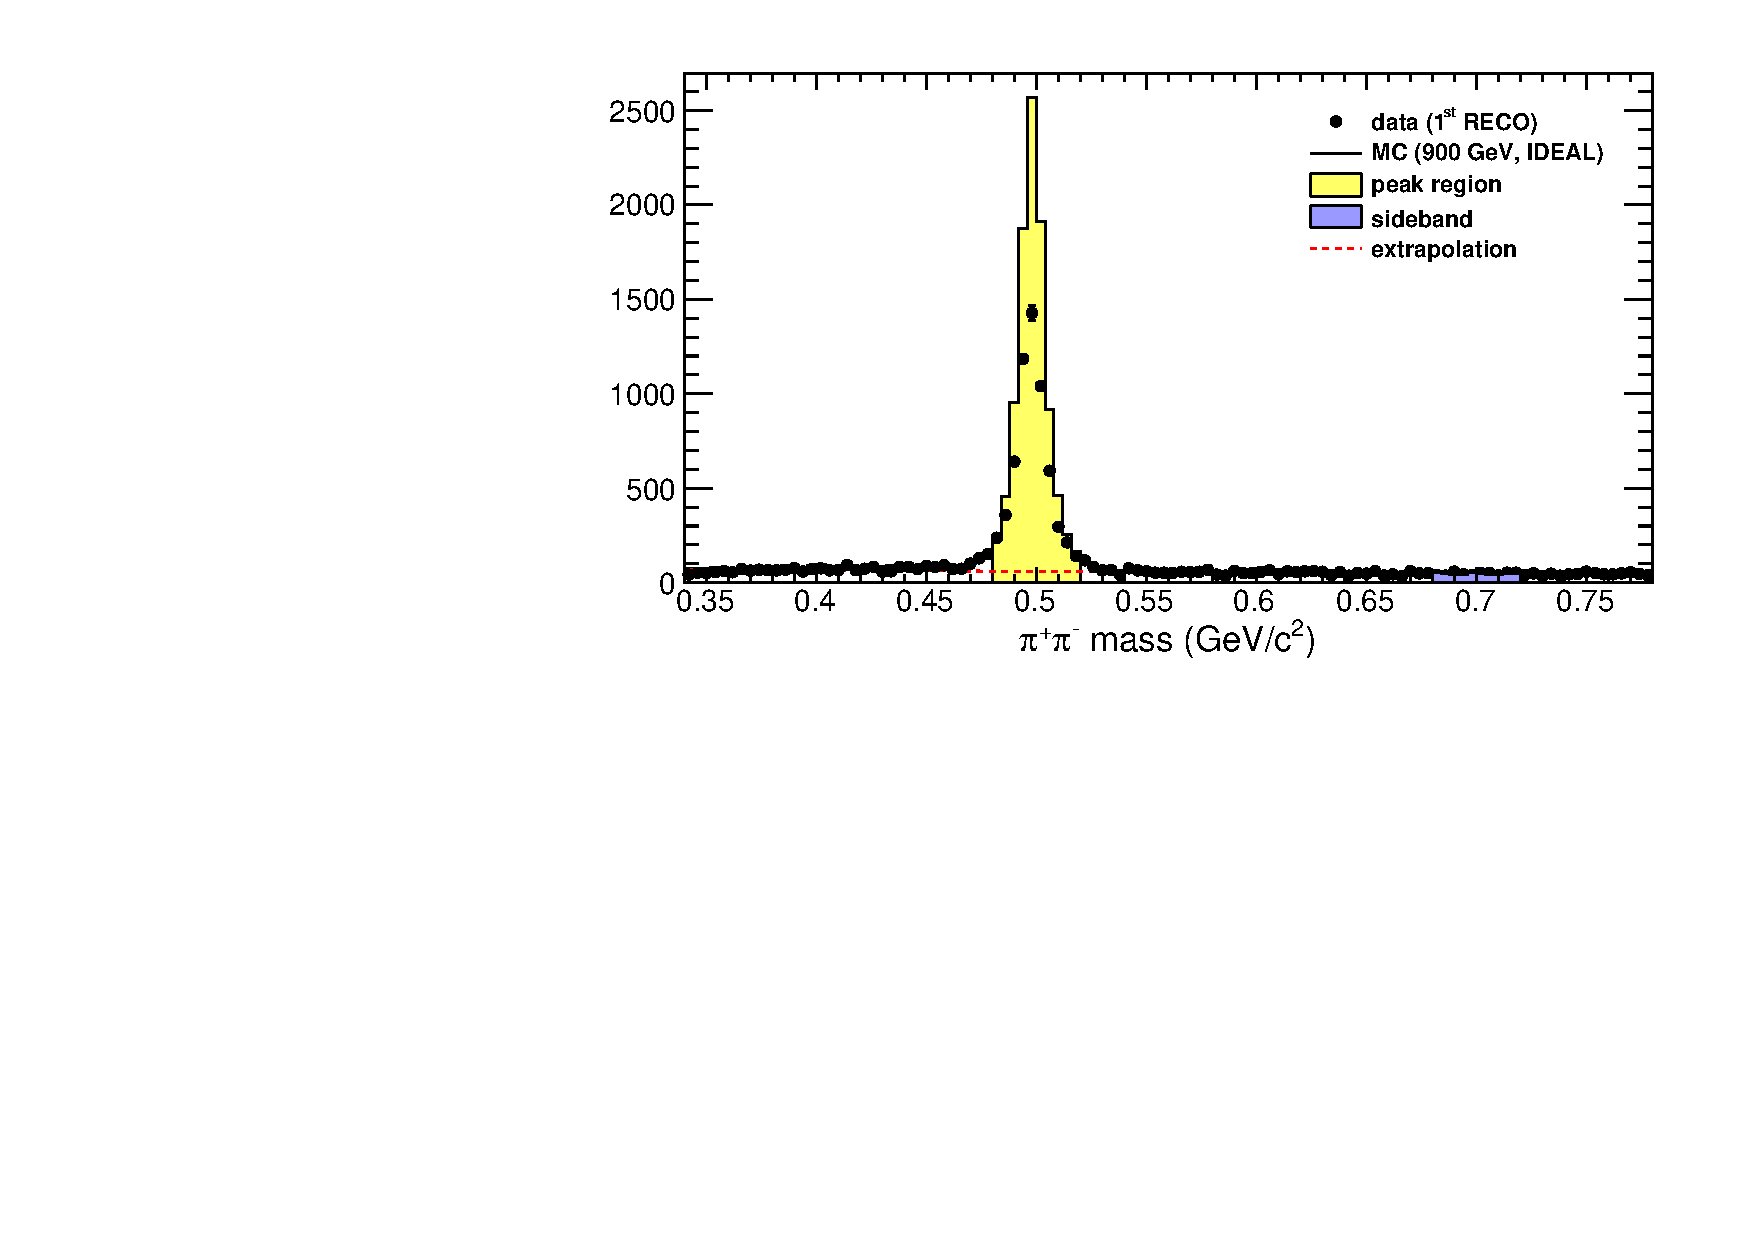
\includegraphics[width=\linewidth]{kaonTracking_masspeak.pdf}

\begin{itemize}
\item Upper sideband only: there can be signal events below peak due
  to final state radiation
\end{itemize}
\end{frame}

\begin{frame}
\frametitle{Feasibility study (2/6)}
\begin{itemize}
\item All plots from this point onward are background-subtracted and
  normalized within cut windows

\item ``MC truth'' is matched to true $K_S$ in MC (no sideband subtraction)
\begin{center}
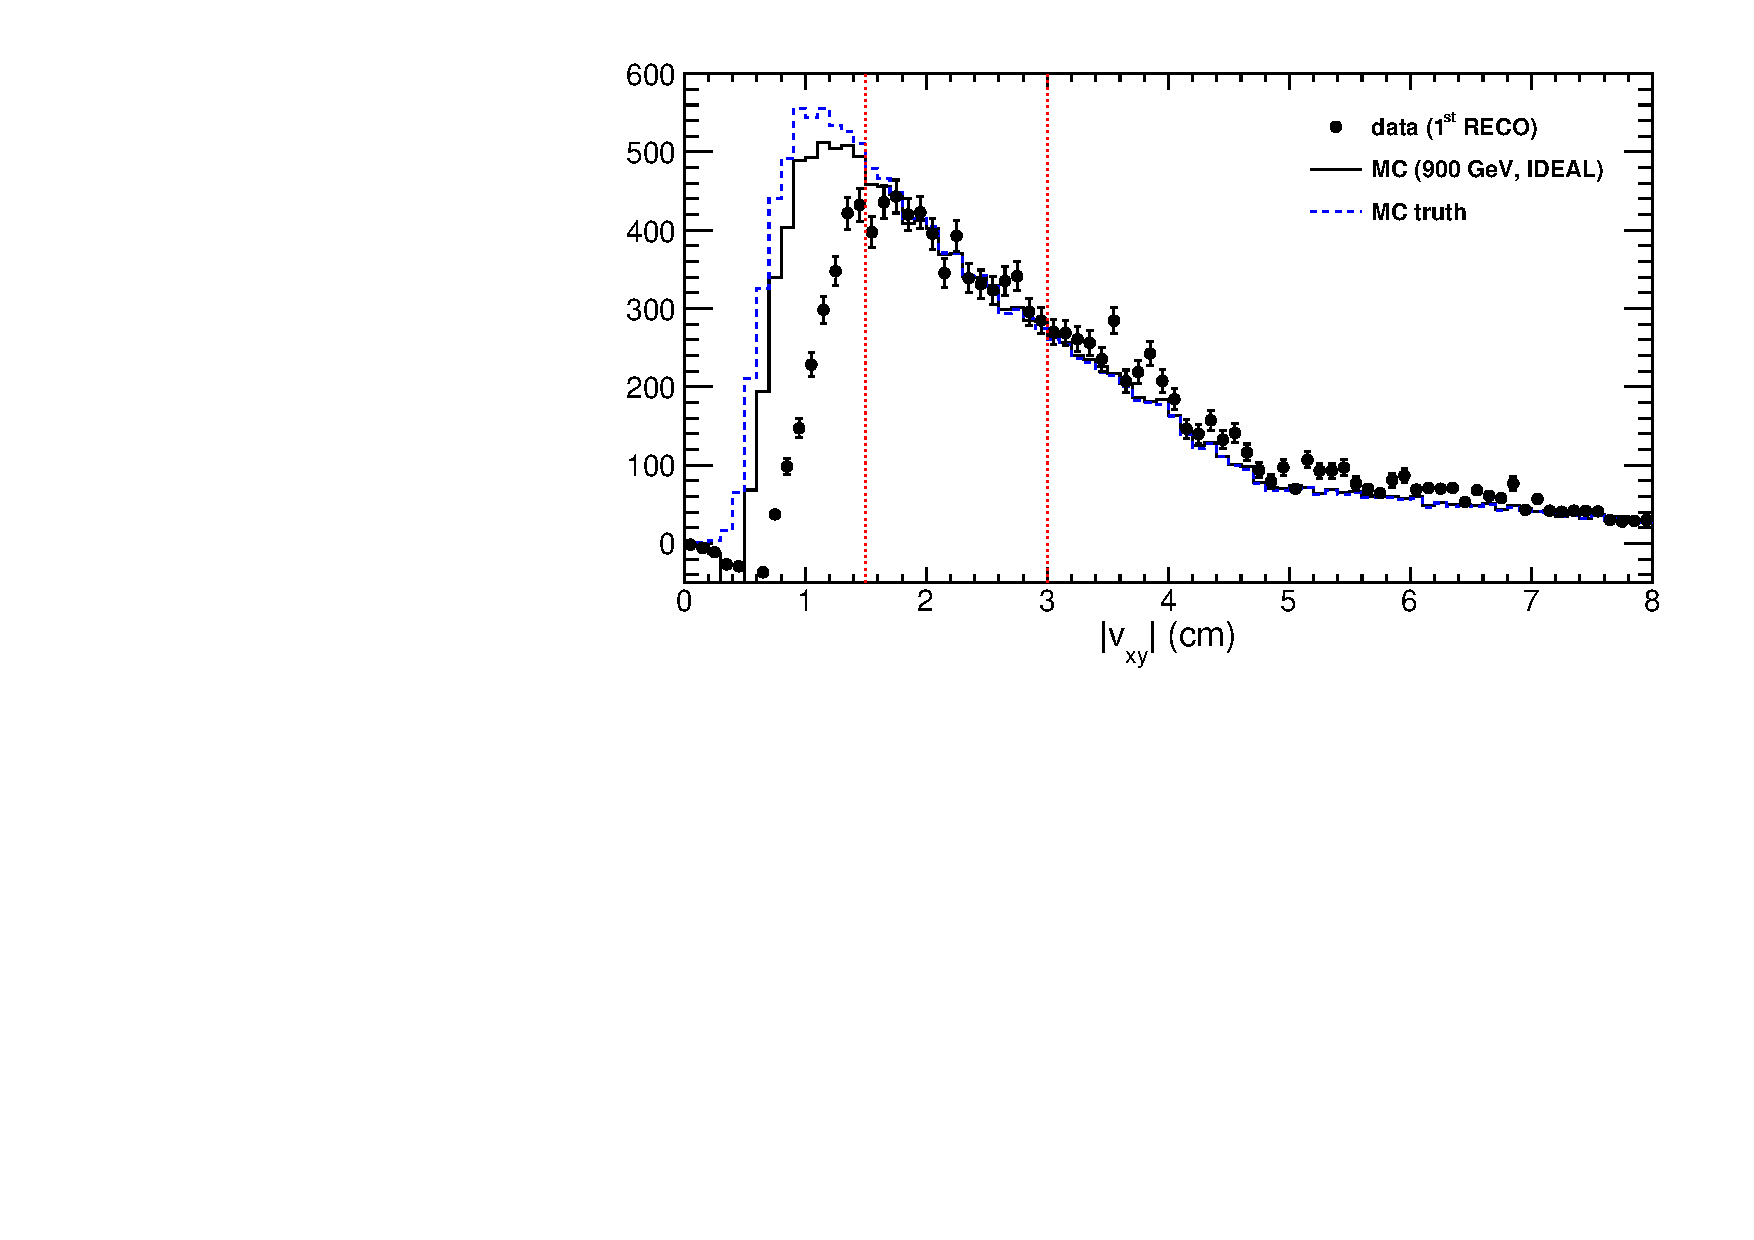
\includegraphics[width=0.9\linewidth]{kaonTracking_vxy.pdf}
\end{center}

\item Could loosen track flight significance and lower $|v_{xy}|$ boundary

\item Upper $|v_{xy}|$ boundary must be within first pixel layer so that resolution is smooth as a function of track $d_{xy}$
\end{itemize}
\end{frame}

\begin{frame}
\frametitle{Feasibility study (3/6)}

\begin{itemize}
\item Propagation of $K_S$ to beamline in two cases: when there is only one primary vertex (left), and when there is also a second (right)

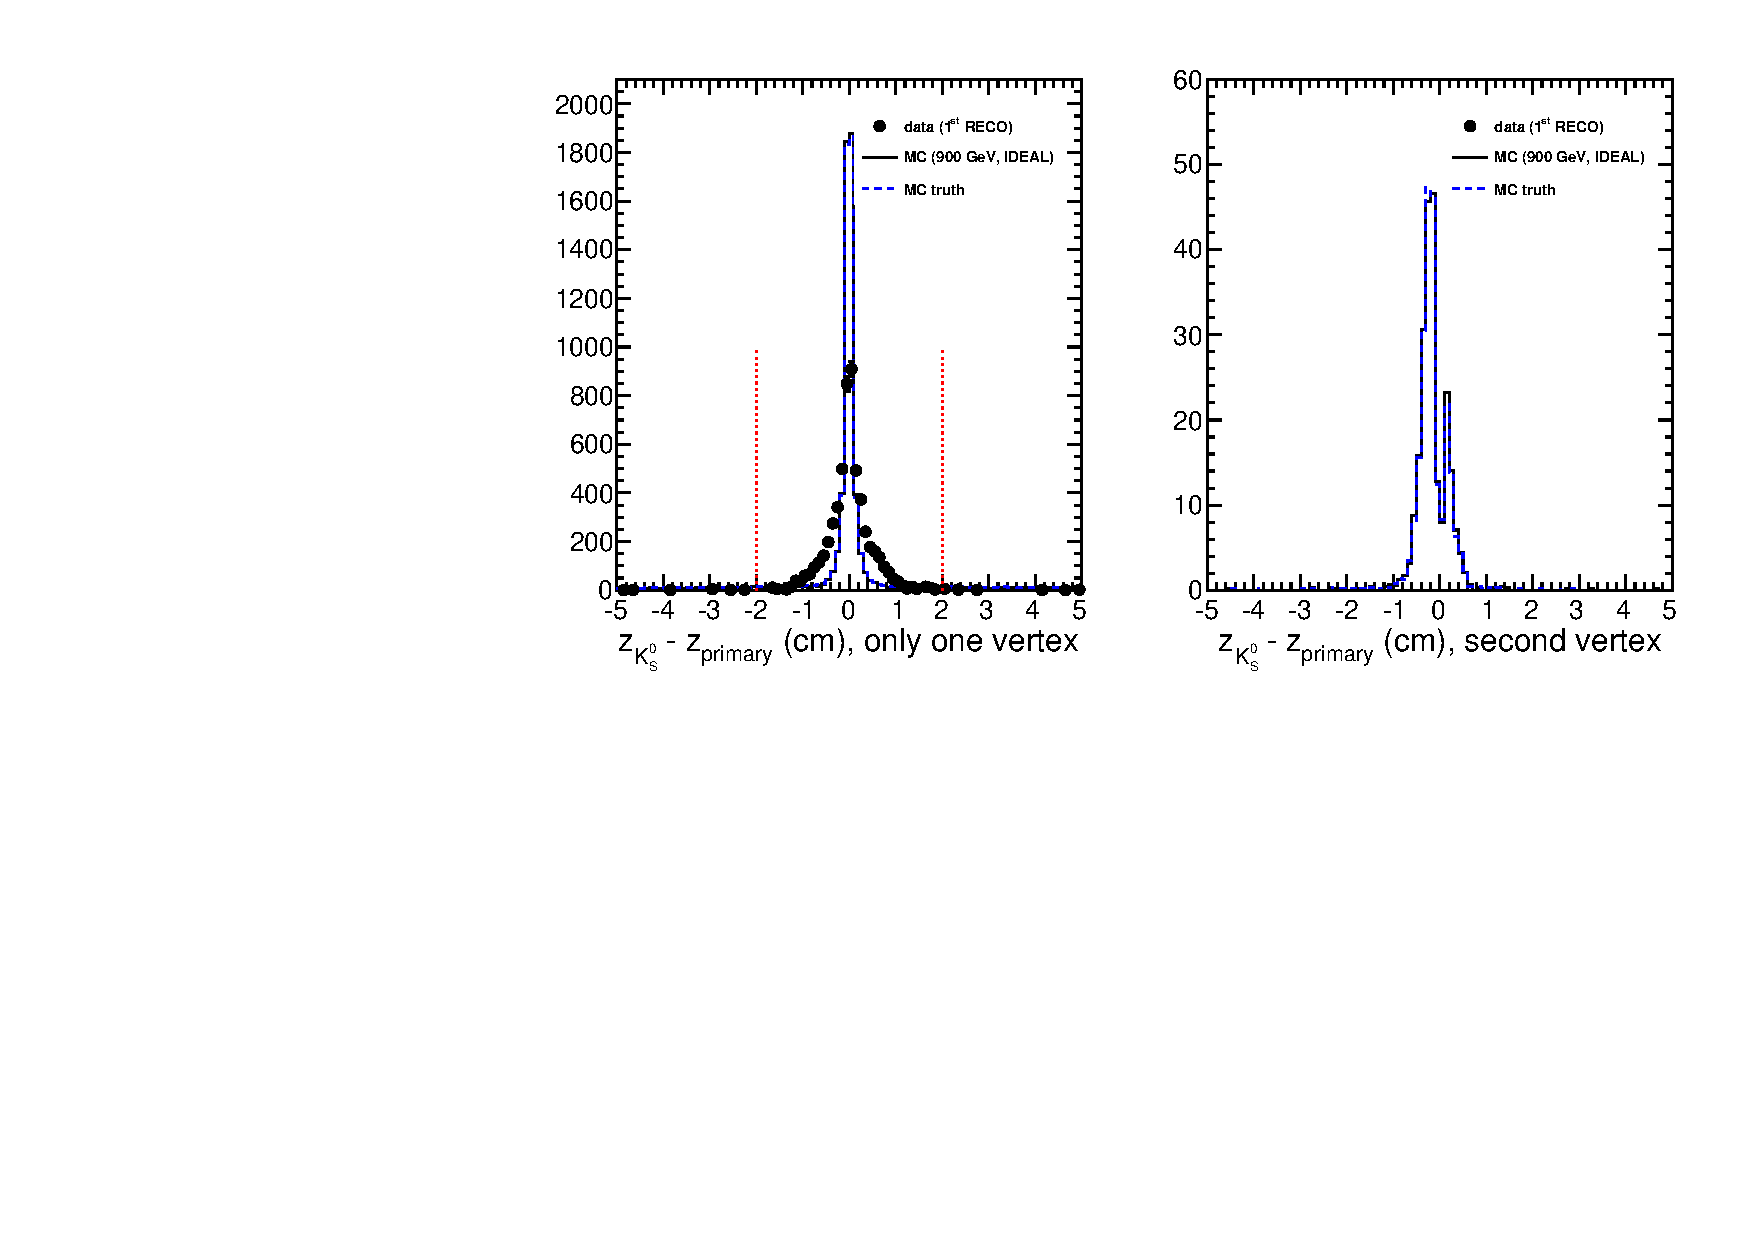
\includegraphics[width=\linewidth]{kaonTracking_zcut.pdf}

\item In MC, 3.4\% of events have a second primary vertex, in data, several do, but well beyond 5~cm (negligible pile-up plus beam-gas?)

\item Efficiency of ``only one vertex'' requirement is \mbox{dependent on luminosity\hspace{-1 cm}}
\end{itemize}
\end{frame}

\begin{frame}
\frametitle{Feasibility study (4/6)}
\begin{itemize}
\item Distribution of all $\Delta \phi$ is not Gaussian: is quadratic
  $\chi^2$ the right estimator?  Does the minimization need to be made
  non-linear (replace $99\times 99$ matrix inversion with Minuit)?

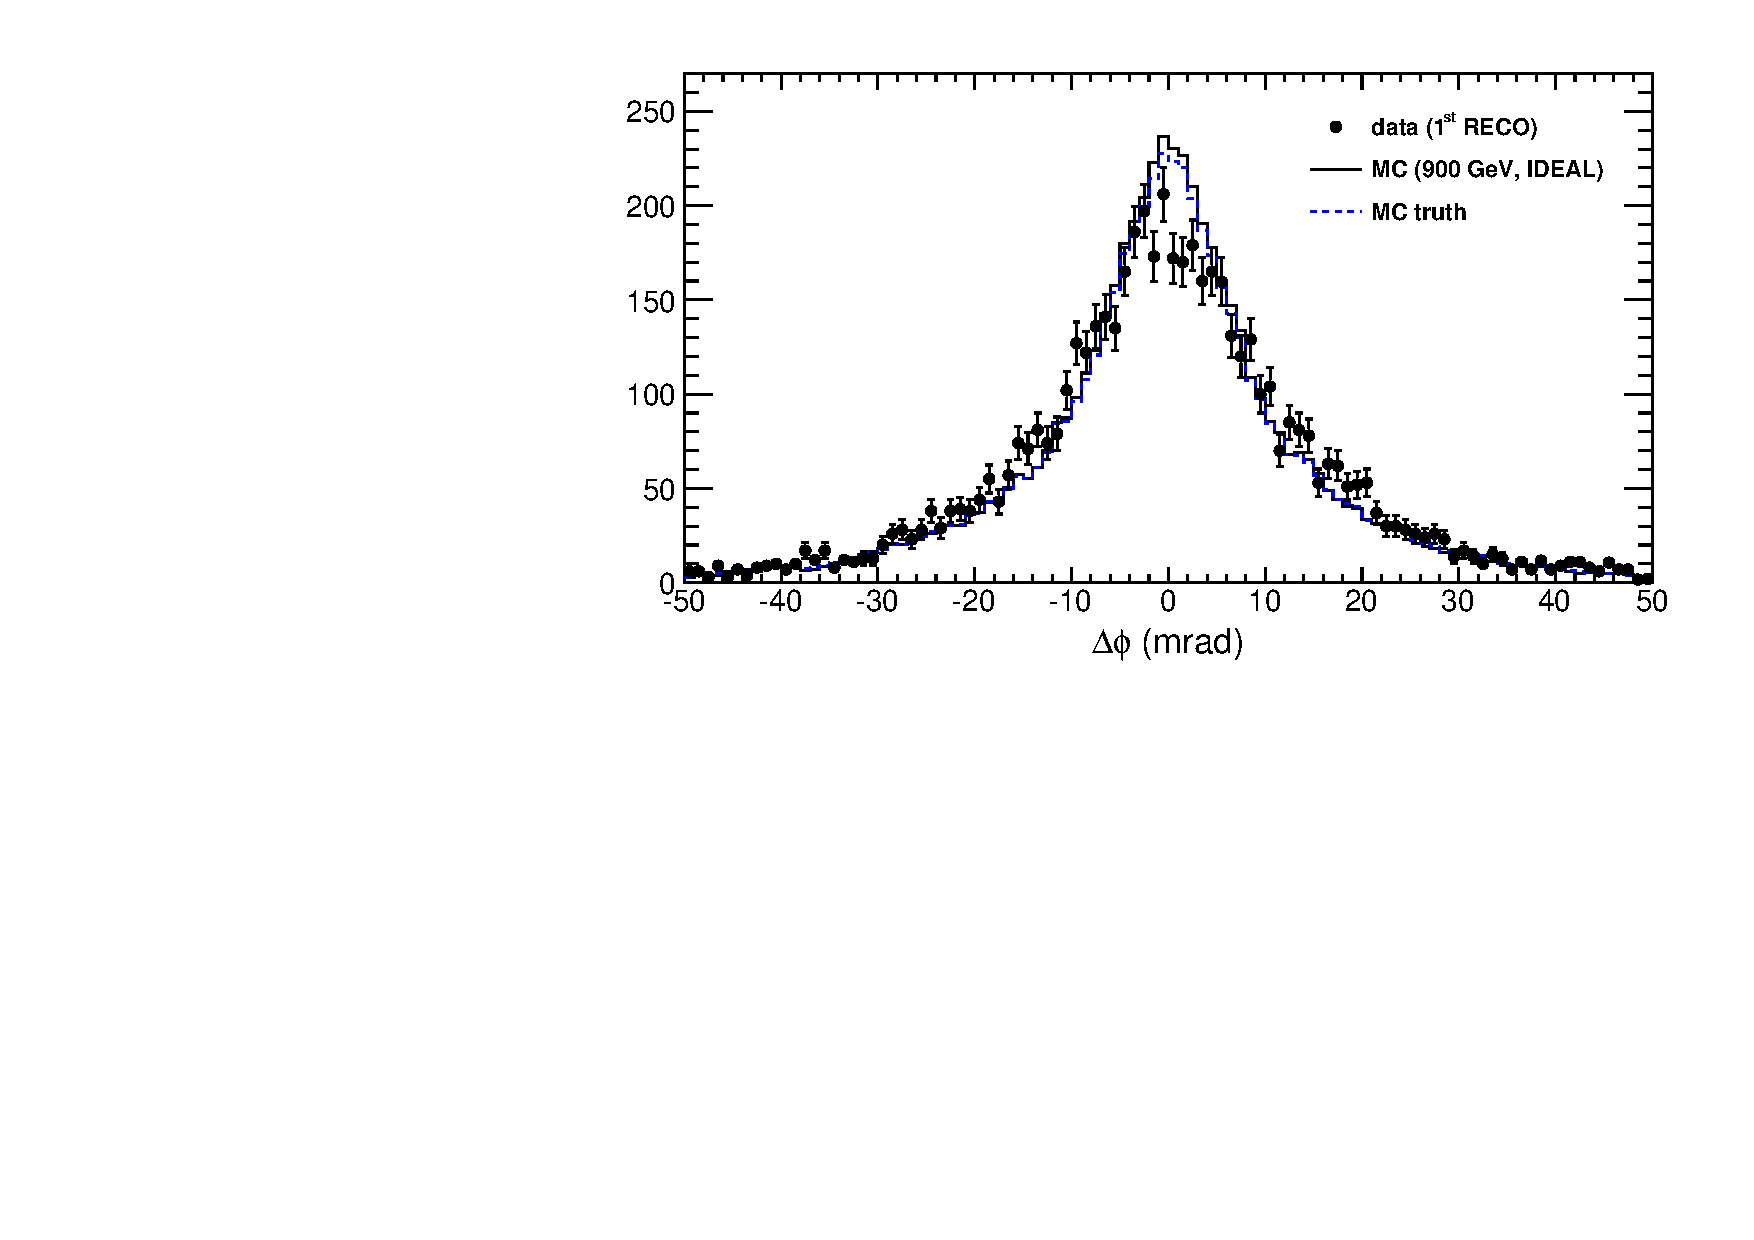
\includegraphics[width=\linewidth]{kaonTracking_deltaphi.pdf}

\item Some indication of $\Delta \phi$ variation in data?  Remember, these are unrealistic APEs
\end{itemize}
\end{frame}

\begin{frame}
\frametitle{Feasibility study (5/6)}
\begin{itemize}
\item Calculation of ${\sigma_{\Delta \phi}}^2$ weights must include
  all correlations between two-track intersection and momentum sum,
  starting from $5\times 5$ track parameter covariances

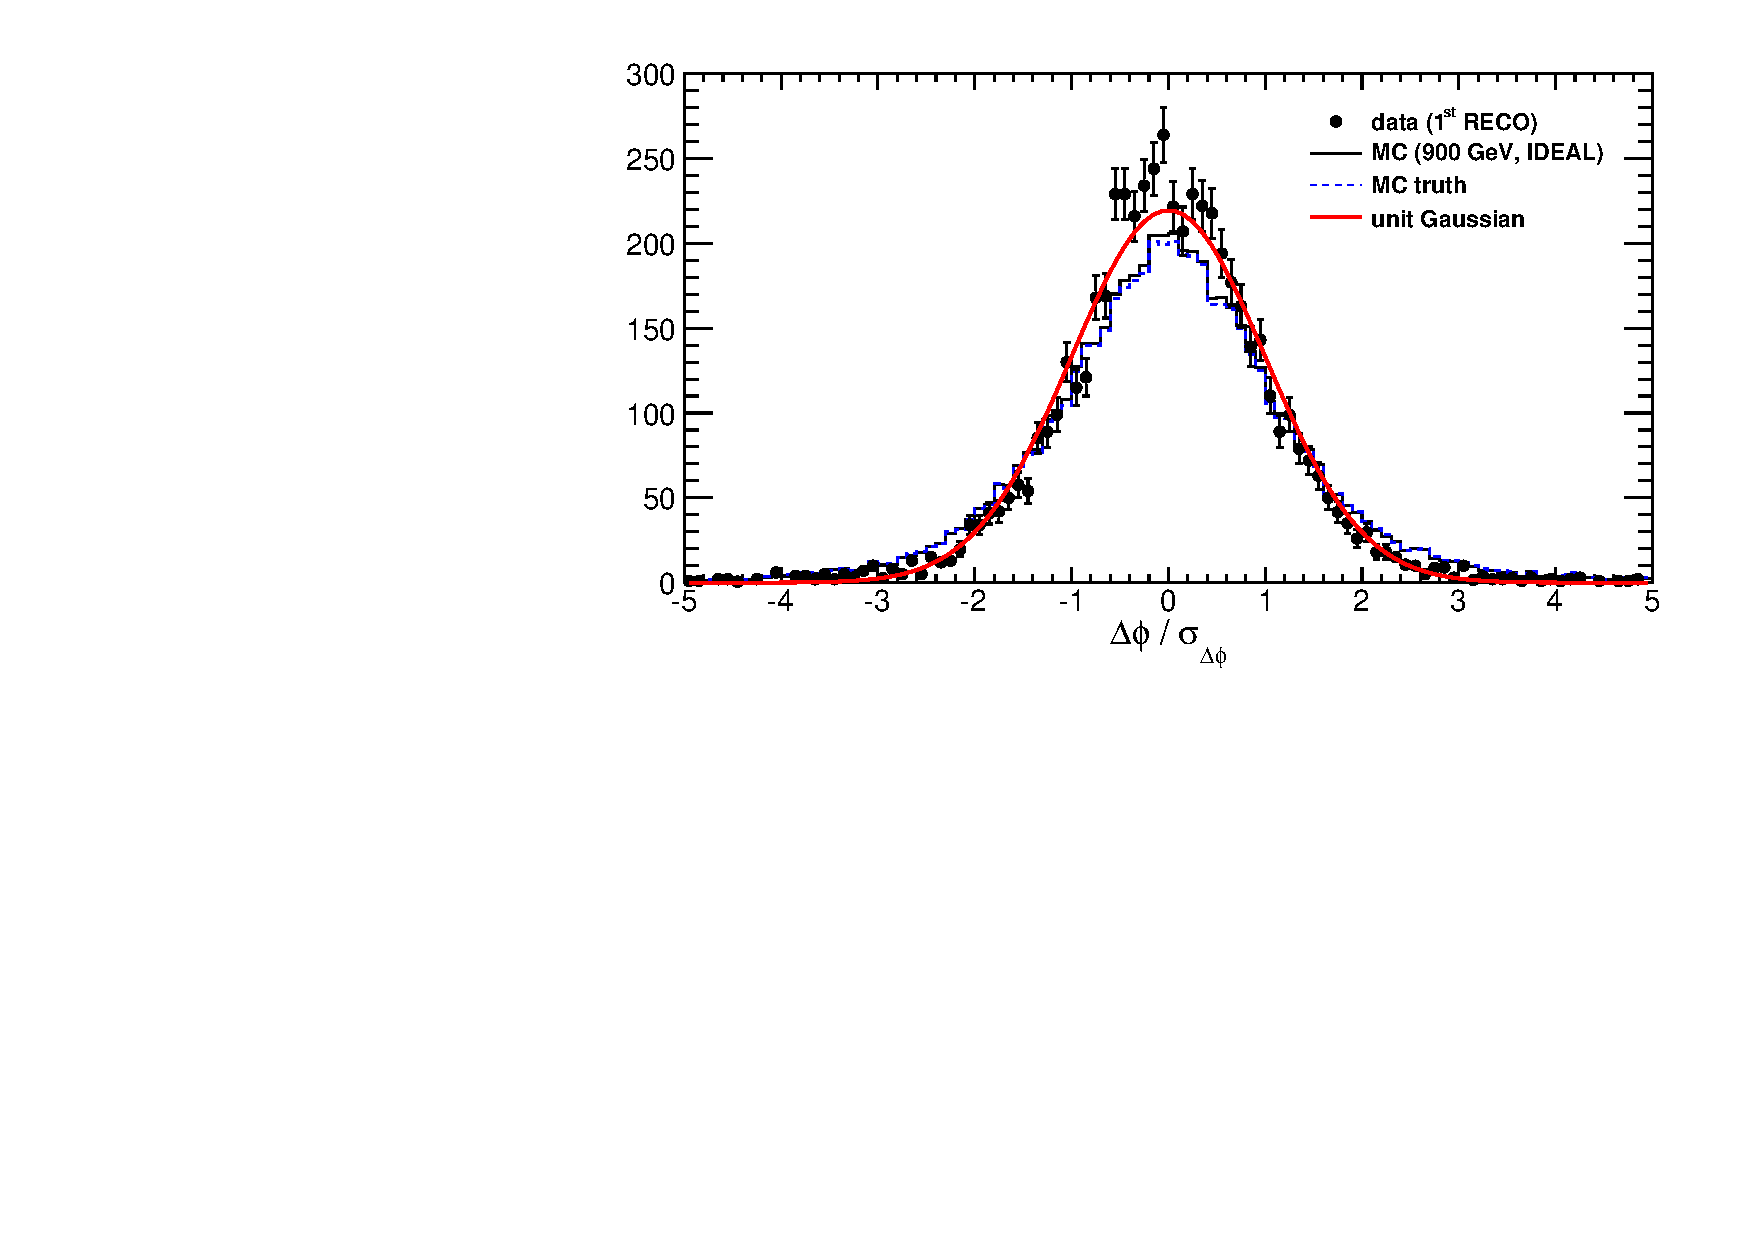
\includegraphics[width=\linewidth]{kaonTracking_normalized.pdf}

\item Uncertainty is slightly underestimated in MC, larger in data

\end{itemize}
\end{frame}

\begin{frame}
\frametitle{Feasibility study (6/6)}
\begin{itemize}
\item $\Delta \phi$ histogram weighted by $1/{\sigma_{\Delta \phi}}^2$

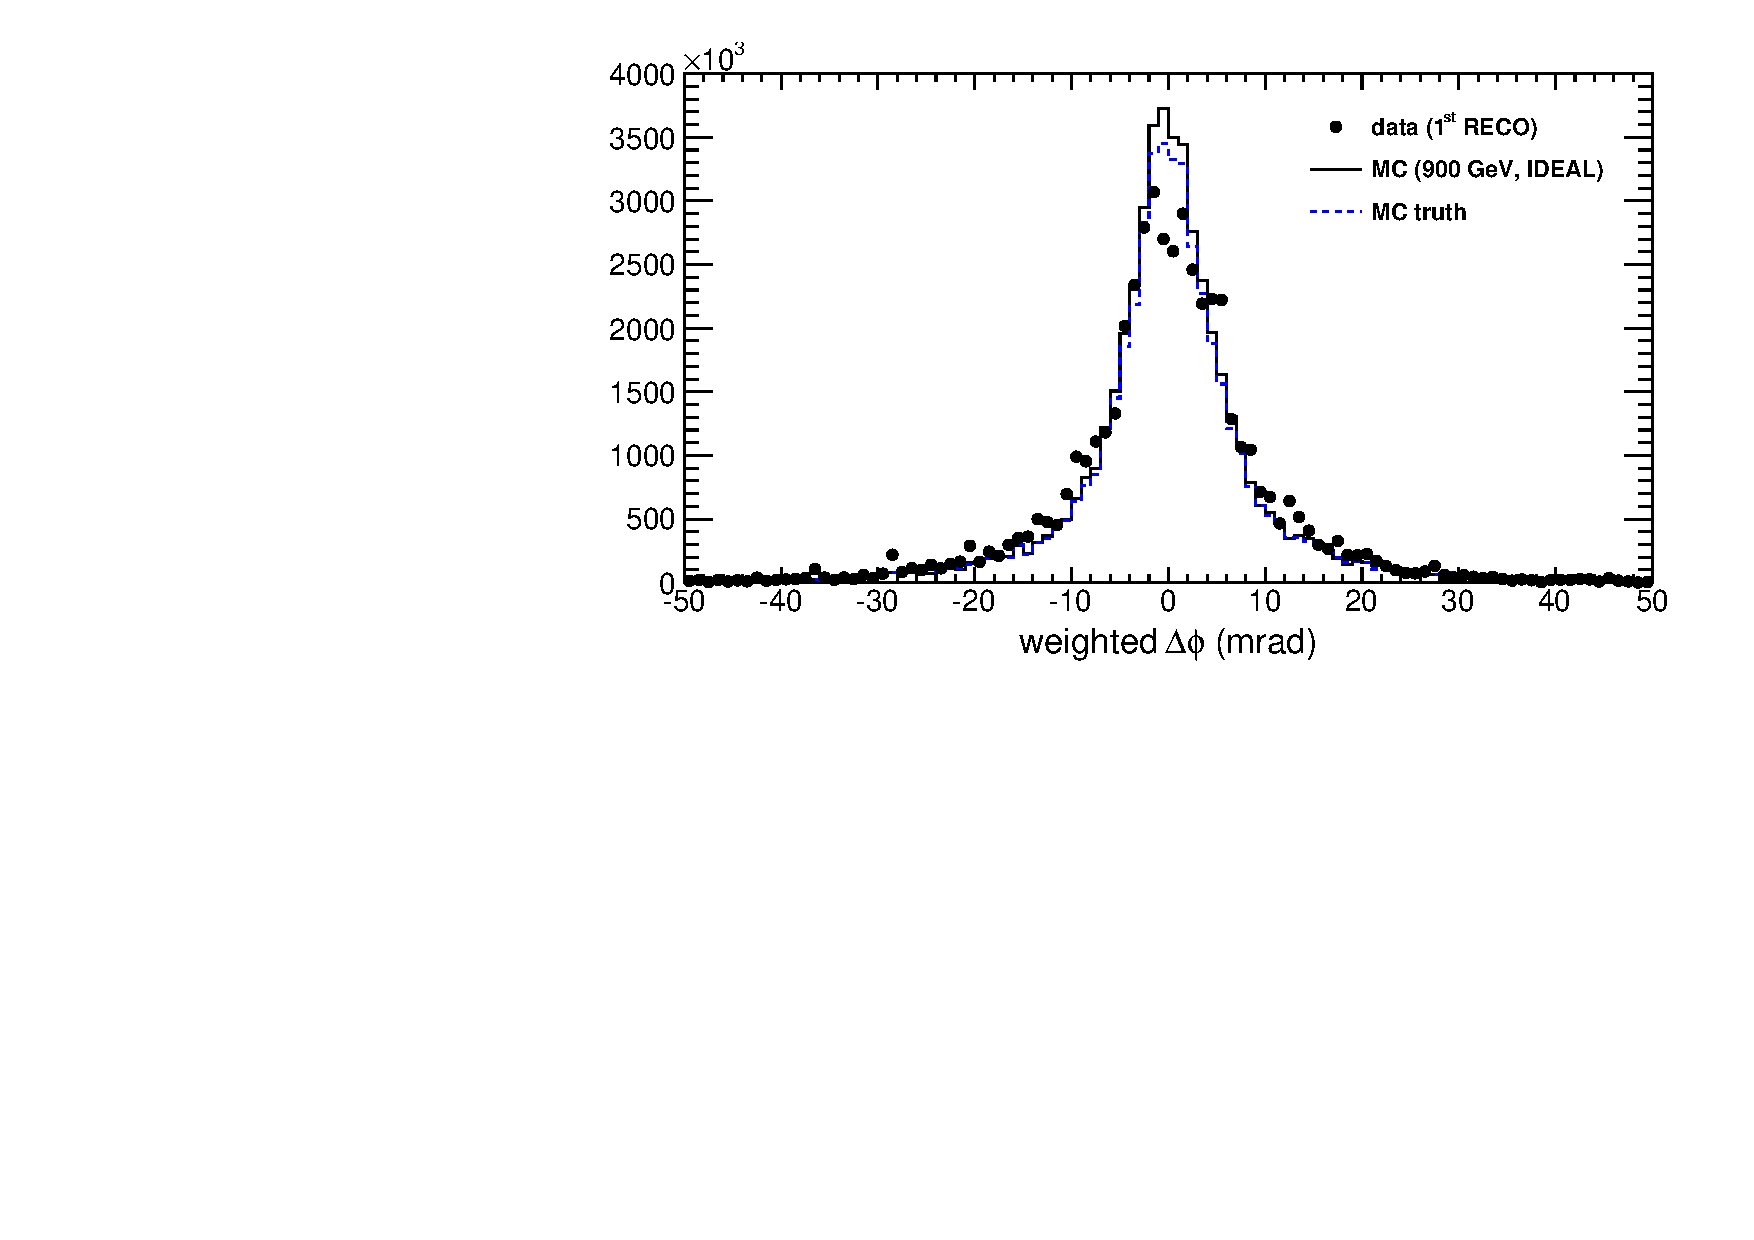
\includegraphics[width=\linewidth]{kaonTracking_weighted.pdf}

\item Much narrower, indicating that the largest outliers have the largest uncertainties

\item Data are still broader than MC (and distribution still not Gaussian)
\end{itemize}
\end{frame}

\begin{frame}
\frametitle{Conclusions}
\begin{itemize}
\item Proposal: multi-step track corrections
\begin{enumerate}
\item alignment corrects track shapes, but can allow relative biases
  in regions of the tracker that are not connected by cosmic rays or
  collisions (assuming no resonance constraints)
\item parameterize track parameter space and apply regional
  corrections to make momentum scale uniform, and also acquire matrix
  of uncertainties
\item apply overall correction to set momentum scale with resonance
  masses, also with uncertainties
\end{enumerate}

\item Even if no track parameter biases are observed, uncertainty in
  bias is an important systematic for physics analyses
\begin{itemize}
\item early analysis: CMS can improve $\Xi^\pm$ mass measurement in an
  analysis with only one systematic uncertainty--- tracking
\end{itemize}

\item Demonstrated selection and $\Delta \phi$, ${\sigma_{\Delta
    \phi}}^2$ calculation \mbox{with $K_S \to \pi^+\pi^-$\hspace{-1 cm}}
\begin{itemize}
\item next steps would be to calculate $\vec{p}$ and its correlations;
  is it consistent with zero in MC?  How much uncertainty per $\sqrt{N}$?
\end{itemize}

\item For most analyses, a higher-mass metastable particle would be
  more relevant: $B \to$ all charged hadrons?

\end{itemize}
\label{numpages}
\end{frame}

\end{document}
